\documentclass{article}
\usepackage{tikz}
\usetikzlibrary{graphs, graphs.standard, quotes}

\begin{document}

\begin{figure}[h]
    \centering
    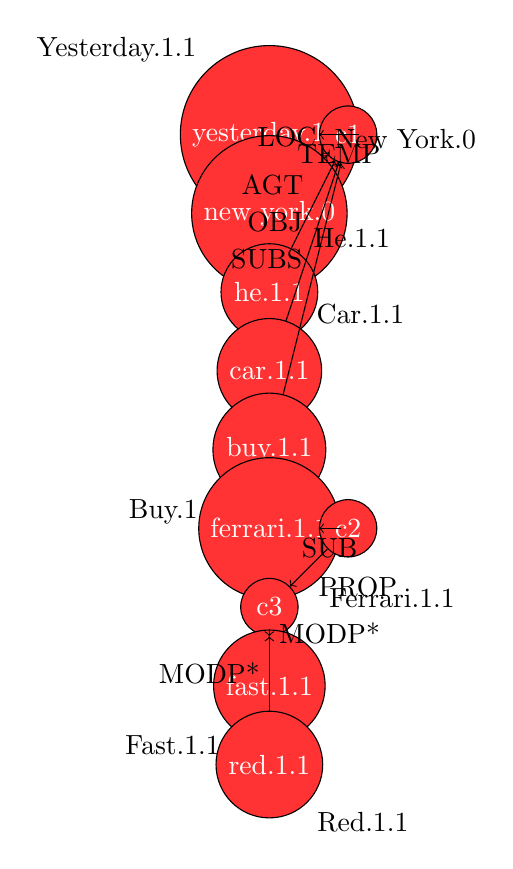
\begin{tikzpicture}
        \graph [simple, nodes={circle, draw, fill=red!80, text=white}, edges={->}] {
            "yesterday.1.1" [label=above left:Yesterday.1.1] -> ["TEMP"] "c1",
            "new york.0" [label=above right:New York.0] -> ["LOC"] "c1",
            "he.1.1" [label=above right:He.1.1] -> ["AGT"] "c1",
            "car.1.1" [label=above right:Car.1.1] -> ["OBJ"] "c1",
            "buy.1.1" [label=below left:Buy.1.1] -> ["SUBS"] "c1",
            "ferrari.1.1" [label=below right:Ferrari.1.1] -> ["SUB"] "c2",
            "c2" -> ["PROP"] "c3",
            "fast.1.1" [label=below left:Fast.1.1] -> ["MODP*"] "c3",
            "red.1.1" [label=below right:Red.1.1] -> ["MODP*"] "c3"
        };
    \end{tikzpicture}
    \caption{Example for a random walk (yesterday.1.1 \textsc{temp}$^{-1}$ \textsc{obj} \textsc{prop} \textsc{modp*} red.1.1) in the SN.}
    \label{fig:random_walk_example}
\end{figure}

\end{document}